\section{Instruction Sets}

\subsection{More on Instruction Format}
\label{sec:instruction-format-extended}

\subsubsection{Arithmetic \& Logical Instructions}

\textbf{Arithmetic} operations treat operands as numbers and have to consider the sign
of the operands. Arithmetic shifts are equivalent to multiplication (left shift) or
division (right shift) by 2 with remainders shifted out. The new bits are filled with
sign bits on the left, and 0's on the right.

\textbf{Logical} operations treat operands as bit patterns. Logical shifts simply discard
the bits shifted out and replenish the new bits with 0's.

There are also \textbf{rotate} operations, which put the bits shifted out back into the
other end of the number.

\subsubsection{Procedures \& Function Calls}

A procedure consists of multiple instructions that are executed in sequence. Within
a procedure, instructions can be given to execute another procedure. For the CPU
to know where to go and where to return after the called procedure is done, the
return addresses need to be stored, which is done by a stack. The latest return
address will be at the top of the stack, and the CPU will pop it when it reaches
a return instruction.

\subsubsection{Instruction Operands}

In most applications, instructions either have three, two, one, or zero operands
(or addresses). Symbolically, they are represented as:

\begin{table}[H]
    \centering
    \begin{tabular}{|c|c|c|}
        \hline
        \textbf{\# of Operands} & \textbf{Symbolic Representation} & \textbf{Interpretation} \\
        \hline
        3 & \texttt{OP A, B, C} & \texttt{A} $\gets$ \texttt{B OP C} \\
        2 & \texttt{OP A, B} & \texttt{A} $\gets$ \texttt{A OP B} \\
        1 & \texttt{OP A} & \texttt{AC} $\gets$ \texttt{AC OP A} \\
        0 & \texttt{OP} & \texttt{T} $\gets$ \texttt{(T-1) OP T} \\
        \hline
    \end{tabular}
\end{table}

{\footnotesize Note: 
\texttt{AC} = accumulator, \texttt{T} = top of stack, \texttt{(T-1)} = second element of the stack
}

Instruction operands can either be in main memory or in registers.

\subsubsection{Registers}

\begin{itemize}
    \item \textbf{General Purpose Registers}: registers that can be used freely;
    \item \textbf{Dedicated Purpose Registers}: e.g. program counter (PC), instruction register (IR), stack pointer (SP), processor status word (PSW), flag register;
\end{itemize}

\subsubsection{Data Types}

Two types of data types: \begin{enumerate*}[label=\textbf{(\arabic*)}]
    \item Numeric (integer, floating point);
    \item Non-numeric (character, binary data).
\end{enumerate*}
The lengths are typically 8, 16, 32, or 64 bits.

For MIPS architecture (a family of reduced instruction set computer (RISC), not ARM or x86),
have 9 basic data types: \begin{enumerate*}[label=\textbf{(\arabic*)}]
    \item signed and unsigned bytes;
    \item signed and unsigned half-words;
    \item signed and unsigned words;
    \item double words;
    \item single-precision floating point (32 bits);
    \item double-precision floating point (64 bits)
\end{enumerate*}.

For ARM architecture, it supports datatypes of \begin{enumerate*}[label=\textbf{(\arabic*)}]
    \item byte (8 bits);
    \item half-word (16 bits); and
    \item word (32 bits)
\end{enumerate*} in length.
It only provides unsigned integers, nonnegative integers, and two's complement integers. 
The ARM architecture does not provide floating point hardware and they must be emulated in
software.

\subsection{Addressing Modes}

\begin{figure}[H]
    \centering
    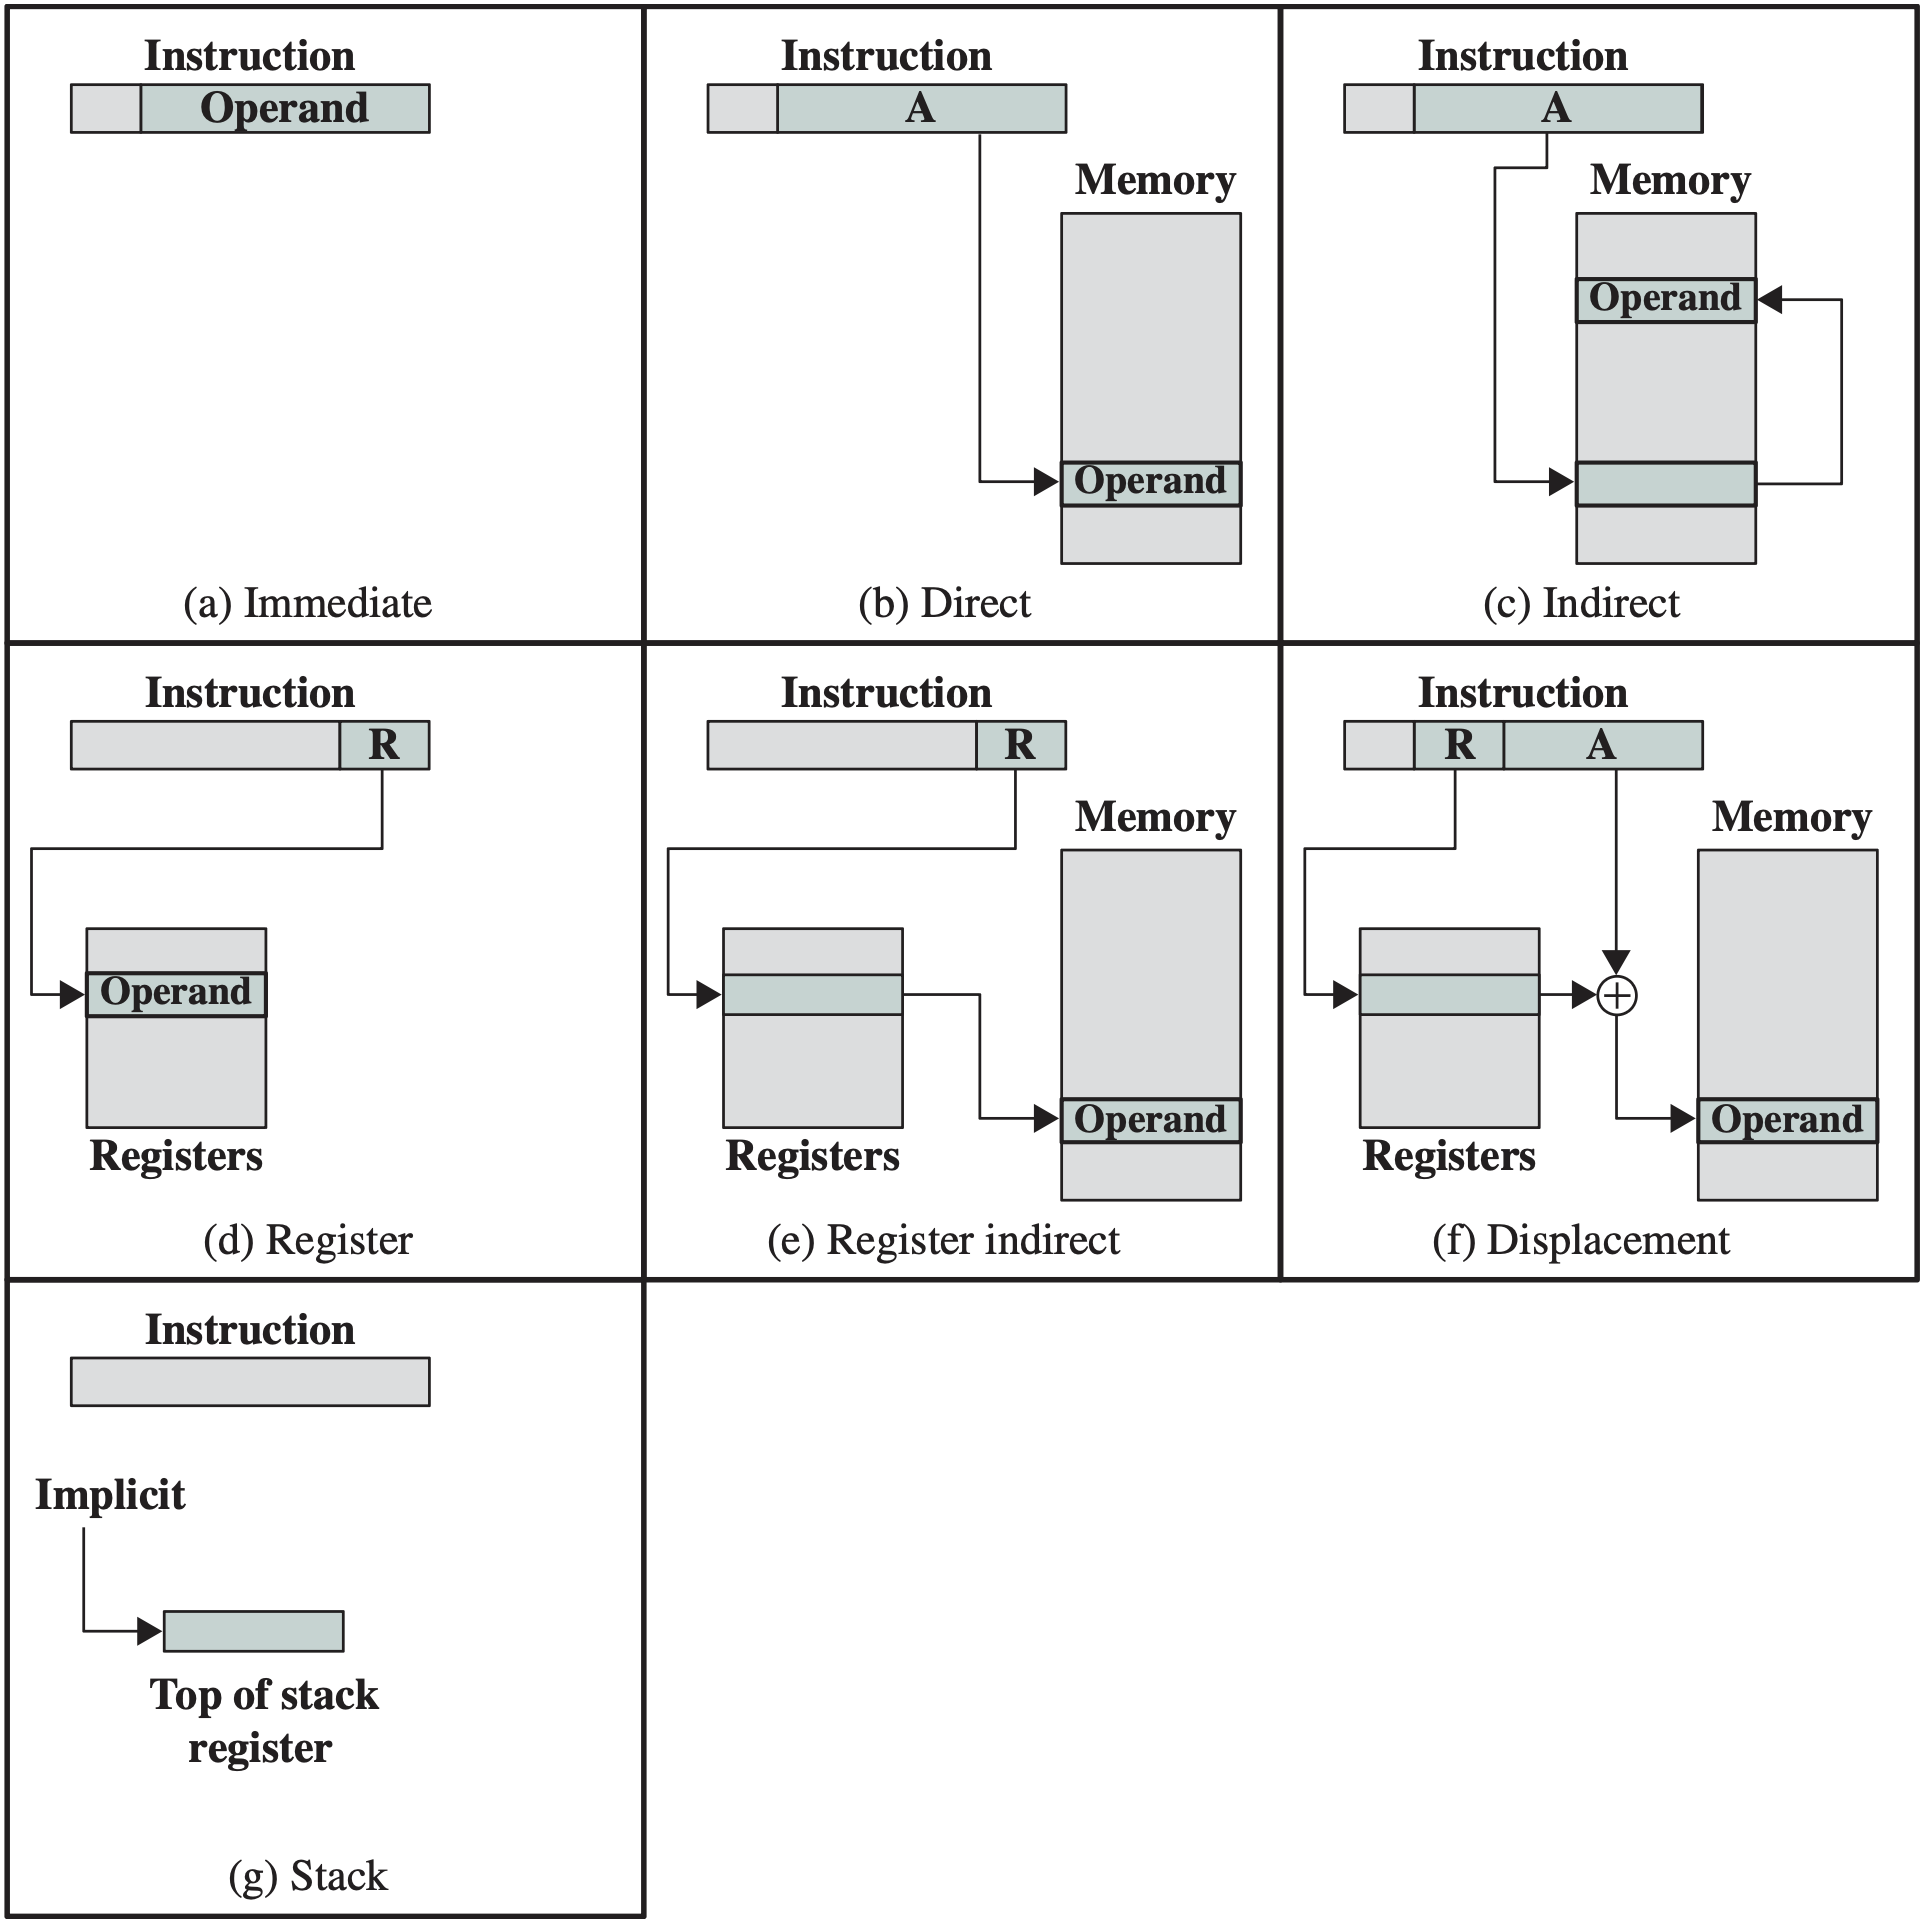
\includegraphics[width=0.8\textwidth]{chaps/instructions-sets/addressing-modes.png}
    \caption{Addressing Modes}
\end{figure}

\begin{remark}
    Notations used in this section:
    \texttt{A} = contents of an address (operand) field of an instruction;
    \texttt{R} = contents of an address field that refers to a register;
    \texttt{EA} = effective address (actual address) of the location where the referenced operand is stored;
    \texttt{(X)} = contents of memory location or register \texttt{X}.

    (The parenthesis notation is similar to a dereference operator of a pointer in C/C++.)
\end{remark}

\begin{multicols}{3}

\subsubsection{Immediate}

\begin{itemize}
    \item \textbf{Notation}: Operand $=$ \texttt{A}
    \item \textbf{Advantage}: No memory references needed.
    \item \raggedright\textbf{Disadvantage}: Limited operand magnitude.
\end{itemize}

\subsubsection{Direct}

\begin{itemize}
    \item \textbf{Notation}: \texttt{EA} $=$ \texttt{A}
    \item \textbf{Advantage}: Simple and increased operand magnitude.
    \item \textbf{Disadvantage}: Limited address space. (Range of memory addresses
        accessible to the instruction depends on the size of the address field.)
\end{itemize}

\columnbreak

\subsubsection{Indirect}

\begin{itemize}
    \item \textbf{Notation}: \texttt{EA} $=$ \texttt{(A)}
    \item \textbf{Advantage}: Increased address space.
    \item \textbf{Disadvantage}: Multiple memory references needed.
\end{itemize}

\subsubsection{Register}

\begin{itemize}
    \item \textbf{Notation}: \texttt{EA} $=$ \texttt{R}
    \item Similar to direct addressing, but the operand is in a register.
    \item \textbf{Advantage}: Fast access to operands.
    \item \textbf{Disadvantage}: Limited number of registers. (e.g. 32 registers in MIPS)
\end{itemize}

\columnbreak

\subsubsection{Register Indirect}

\begin{itemize}
    \item \textbf{Notation}: \texttt{EA} $=$ \texttt{(R)}
    \item Similar to indirect addressing, but the operand is in a register.
    \item \textbf{Advantage \& Disadvantage}: Same as indirect addressing.
\end{itemize}

\subsubsection{Displacement}

\begin{itemize}
    \item \textbf{Notation}: \texttt{EA} $=$ \texttt{A} $+$ \texttt{(R)}
    \item \textbf{Usage}: Accessing local variables or parameters in a function call,
        or accessing an array.
    \item Registers involved: PC, SP, and base pointer register.
    \item \textbf{Advantage}: Flexible.
    \item \textbf{Disadvantage}: Complex.
\end{itemize}

\end{multicols}

\subsubsection{Stack}

\begin{itemize}
    \item \textbf{Notation}: \texttt{EA} $=$ Top of Stack
    \item Uses the stack pointer register (SP). This is implied in the instruction.
    \item \textbf{Usage}: Mainly for \texttt{PUSH} and \texttt{POP} instructions.
    \item \textbf{Advantage}: No memory reference.
    \item \textbf{Disadvantage}: Limited applicability.
\end{itemize}

\subsection{Assembly Language Programming}